\documentclass[uplatex]{jsarticle}
\usepackage[utf8]{inputenc}

\usepackage{amsmath}
\usepackage[dvipdfmx]{graphicx}
\usepackage{resume}  % resume用スタイル
\usepackage{udline}  % 下線用
\usepackage{comment} % 複数行コメント
\pagestyle{plain}
 
\begin{document}
\twocolumn[
    \beginheader{令和5年度 コンピュータサイエンス学部 中間発表}{2023}{8}{9}{井上 研究室}
    \title{VR環境での落下感に姿勢が与える影響}
    \author{C0B20205 武田 夢音 (Yumene Takeda)}
    \endheader
]
\vspace{3mm}

%%ページ番号
\setcounter{page}{9}

\section{はじめに}
近年,バーチャルリアリティ(以降,VR)機器の高性能化・低廉化に伴い,一般消費者でもVR環境を用いて様々な体験をすることができるようになった.

VRは現実に近い体験をするために用いられることが多く,そのためには現実の再現によって起こる臨場感が必要である.
しかし,一般的なVR機器は落下という感覚に対しての情報提示が視覚と聴覚に対してのみであり,様々な場面を再現し現実に近い臨場感を与えるには物足りない.

そこで,本研究では落下という感覚に注目し視覚と聴覚以外の感覚に働きかけることで臨場感を高めてゆく.

落下をテーマとして選んだ理由は2つあり,まず1つ目は落下はすでに現実のエンターテインメントとしてバンジージャンプやスカイダイビングが存在しており,そのどちらも料金や手間を理由に気軽に体験することことは難しいためVRとして再現する意義があると考えたこと.

そして2つ目は,落下は大きな動きや複雑な動きがないためシステムとして実装することが比較的容易であると考えたためである.

また,落下時の体勢が落下感覚の発生に関わっているという点に着目し,体の角度を自動で機械的に変化させられるデバイスの開発と落下時の体の角度および落下中の角度の変化が落下感覚に与える影響を明らかにすることを目的とする.



\section{関連研究}
東山らの研究\cite{vection}はロールベクション(刺激によって反対方向に回転していると錯覚する効果)に姿勢が与える影響についての分析を行っており,被験者に5種類の体勢を取らせて視覚刺激を与えることで発生するベクションの強度や発生速度についての実験を行っている.結果から,ベクションの知覚が最も早くなるのはうつ伏せと仰向けであり,ベクションが筋肉系の活動状態(姿勢の制御)による影響を受けることが示された.

奥川らの研究\cite{spatial_stimulation_effect_falling}はVR空間における視覚刺激と体勢によって発生する落下感覚の分析を行っており,落下時に見える風景の空間周波数と落下時の体勢を数パターン用意し,それぞれの落下感覚を比較する実験を行った.結果から,空間周波数は高いほど落下感覚が高まり体勢は伏臥位が最も落下感覚が高まるという結果が得られた.


 \begin{figure}[tb]
  % width や height で絶対的な大きさ指定をすることもできる
  \centering
  \fbox{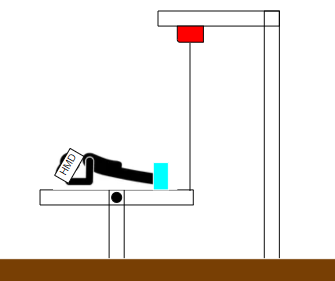
\includegraphics[width=1\linewidth]{fig/main_system.png}}
  \caption{システム概要図}
  \label{fig:about_system}

\end{figure}

\section{角度可変システム}
\subsection{システム概要}
システム概要の図を\figref{fig:about_system}に示す.プレイヤーは頭部にヘッドマウントディスプレイ(以降,HMD)を装着し,上から吊るされた台の上で伏臥位をとる.台の片側はウィンチにつながれており,VRシミュレーション中に体の角度を変えることができる.
仮想空間にはビルの上などの高い場所にいるシチュエーションを用意し,被験者に対して数百メートルの高さから落下する映像を提示できるようにする.
伏臥位になったプレイヤーはVR空間内で落下を体験し,落下に合わせて上下するウィンチによって体の角度が変化する.

\subsection{システム構成}
本研究で使用するウィンチはボタンによる操作を行うため,マイコンを用いてボタンを押すデバイスを作成し間接的に機械制御を行えるようにする.また,マイコンにはArudinoを用いる.

\section{評価方法}
本実験では落下感覚の比較のためマグニチュード法を用いる。

例えば基準となる状態での落下感覚を100として,比較を行いたい状態での落下感覚が半減したと感じたら50,倍程度になったと感じたら200と答えてもらう手法であり,数値にならない感覚の測定を行うのに適した手法である。

基準となる体勢を水平な伏臥位として,そこから15度ずつ下に傾けた体勢を比較対象として評価を行う。
また,実験中に角度を水平から傾けた際の落下感覚の変化も比較を行いたい。

\section{検討事項}
本研究の検討事項は3つある.

1つ目は実験内容についての検討であり,落下時に与える視覚,聴覚,姿勢以外の提示情報は何を提示するかということである.
落下感覚にはこれ以外にも風や振動などが関係していることが分かっている\cite{青木誠也2018音と風によって浮遊感を感じさせる装置の制作}.
そのため、視覚,聴覚,姿勢以外に何の要素を加えてどの程度落下感覚を与えて実験を行うか検討する必要がある.

2つ目も同じく実験内容についての検討であり,シミュレーション中に体を傾ける場合,体を傾けるタイミングについてである.
まだこのシミュレーション自体についての検討が足りていないため,体を傾けるタイミングやこのシミュレーション自体の必要性についても検討が必要である.

3つ目は安全性についてである.
現在作成を考えているデバイスは体を固定する機構を想定しておらず,体を下に傾けすぎた場合にずり落ちてしまうことが容易に想像できる.また,角度変化の際の安全性を考える必要もあるため,それらについて検討する必要がある.

\section{今後の展望}
まず目指すこととして,体を傾けることのできるデバイスが完成しておらず,実験に着手できないためその作成を第一の目標として作業を進める.

\section{まとめ}
本研究ではVR環境で落下する際の体勢の角度の違いによって生じる落下感覚の差について比較と調査を行い,今後はデバイスの作成と実験を行う予定である.


 \bibliographystyle{junsrt}
\bibliography{ref.bib}   % 参考文献のデータベースファイルを指定する 
\end{document}
